% \subsection{Data Products and Expected Return}
% ===============================================================================================================================
\begin{frame}{Gamma-ray bursts}
  \begin{columns}
    \begin{column}{0.6\textwidth}
      \begin{overprint}
        \onslide<1-2>
        \uncover<1->{
        \begin{itemize}
          \item [] Spectra:
          \begin{itemize}
            \item Simulations based on Fermi-LAT data from a few prominent bursts
            \item Selected models are used to account for the effect of EBL
            \begin{itemize}
              \item [\to] Depending on the level of the EBL the number and energy of detected photons can vary significantly
            \end{itemize}
          \end{itemize}
        \end{itemize}
        }

        \uncover<2->{
        \begin{itemize}
          \item [] Light curves:
          \begin{itemize}
            \item Simulations based on Fermi-LAT data extrapolated into CTA band
            \item CTA is capable of resolving the light curves in detail
            \item Energy-dependence of the light curves are of particular value
          \end{itemize}
        \end{itemize}
        }
      \end{overprint}
    \end{column}%
    \begin{column}{0.38\textwidth}
      \begin{overprint}
        \onslide<1>
        \centering
        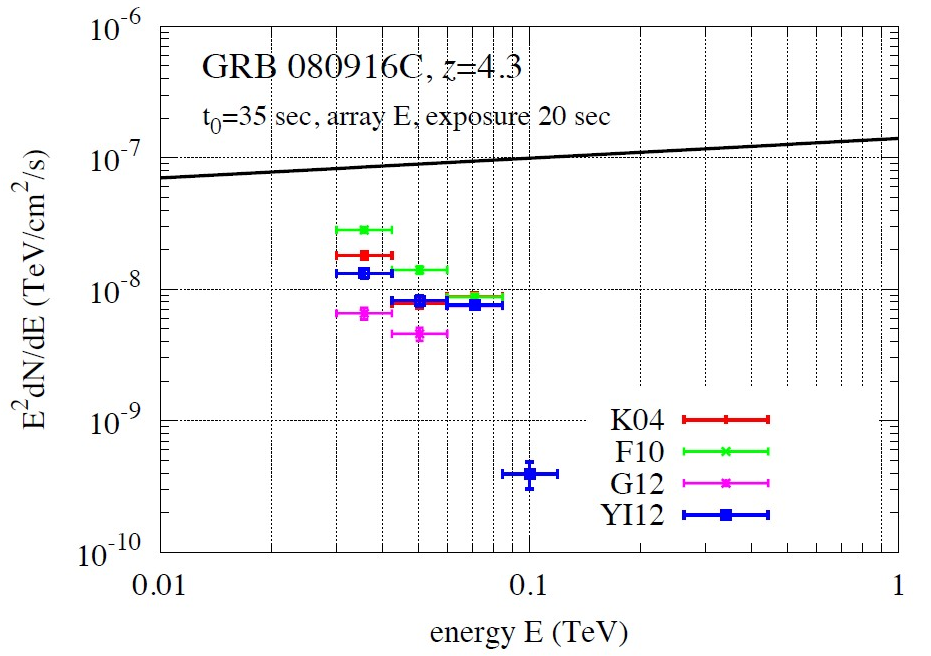
\includegraphics[width=\textwidth]{Plots/grb_sim.png}
        \onslide<2>
        \centering
        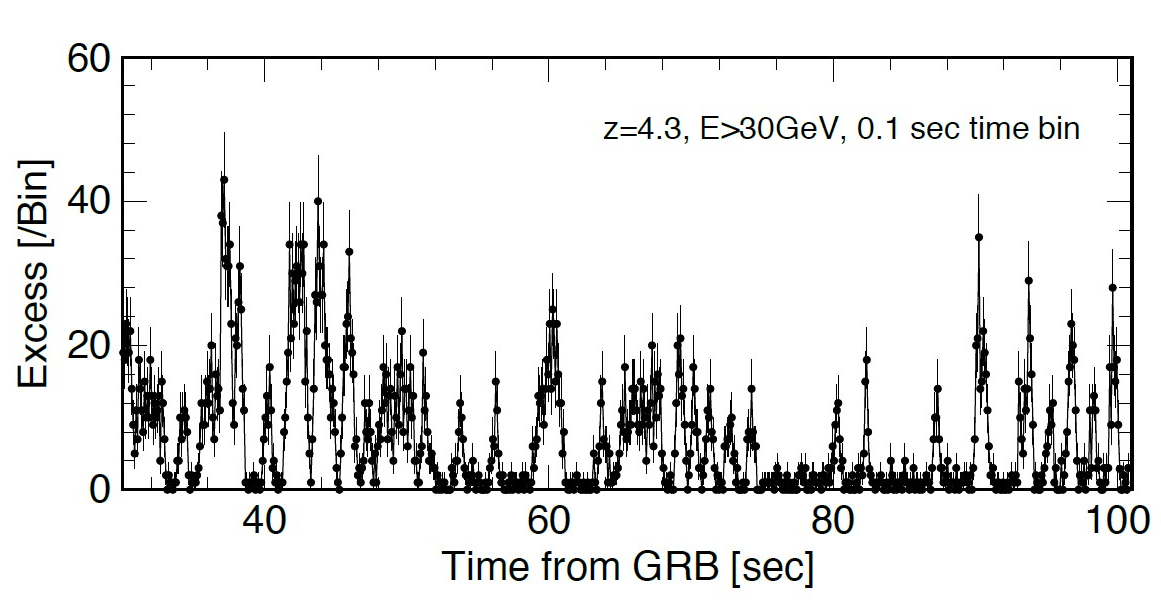
\includegraphics[width=\textwidth]{Plots/grb_sim_lightcurve.png}
      \end{overprint}
    \end{column}%
  \end{columns}
\end{frame}

\begin{frame}{Gamma-ray bursts}
  \begin{itemize}
    \item [] Detection rates:
    \begin{itemize}
      \item Predictions based on a population model tuned to match SWIFT observations
      \item General expecation: order of one CTA detection per year per site
      \begin{itemize}
        \item [\to] Depends on CTAs capability of detecting GRBs with more moderate luminosities
      \end{itemize}
    \end{itemize}
  \end{itemize}
\end{frame}

% ===============================================================================================================================
\begin{frame}{Galactic transients}
  \begin{columns}
      \begin{column}{0.6\textwidth}
        \begin{itemize}
          \item Simulations for Crab nebula HE flares predict observation times of 4 hours per night for $\sim\num{10}$ nights to detect variable inverse-Compton component
          \item CTA could unveil the nature of these flares and constrain the bulk Lorentz factor $\Gamma$
        \end{itemize}
      \end{column}%
      \begin{column}{0.38\textwidth}
        \centering
        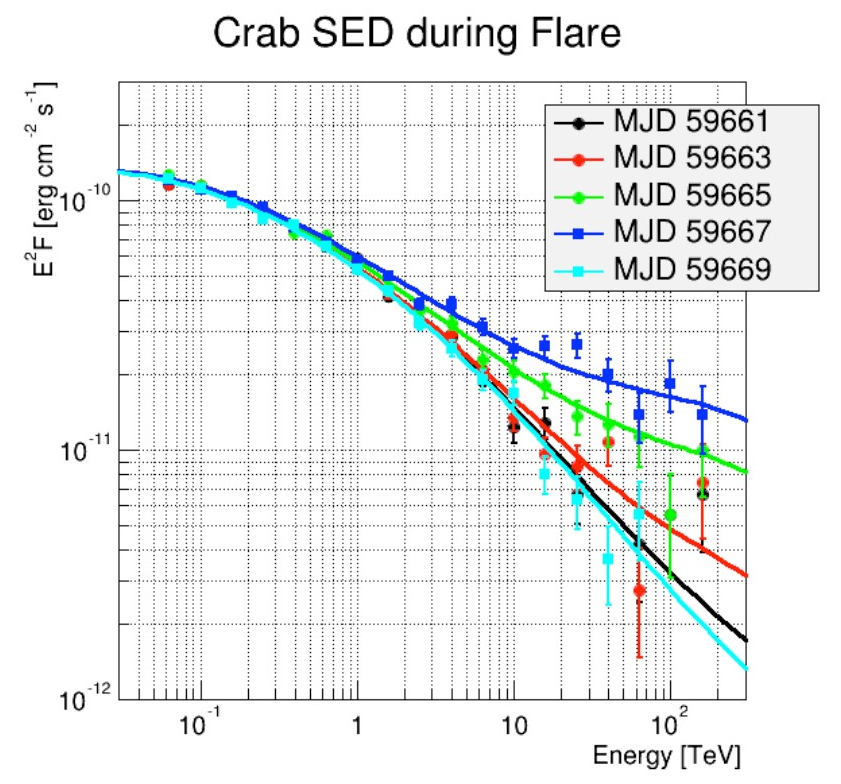
\includegraphics[height=0.85\textwidth]{Plots/crab_sim.png}
      \end{column}%
  \end{columns}
\end{frame}

\begin{frame}{Galactic transients}
  \begin{itemize}
    \item [] Cyg X-3:
    \begin{itemize}
      \item With an extrapolated spectrum taken by Fermi-LAT, CTA north could
      \begin{itemize}
        \item [\to] Detect the source at $5\sigma$ in $\sim\num{10}$ hours
        \item [\to] Obtain the spectrum in up to $\num{30}$ hours
      \end{itemize}
      \item Harder spectrum: Signifiant decrease in observation time
    \end{itemize}
    \item [] Cyg X-1:
      \begin{itemize}
        \item [\to] $5\sigma$ detection in 4 minutes
        \item [\to] Good spectrum in $\sim\num{15}$ minutes
      \end{itemize}
  \end{itemize}
  \begin{overprint}
    \begin{minipage}{0.48\textwidth}
      \centering
      \only<1>{
      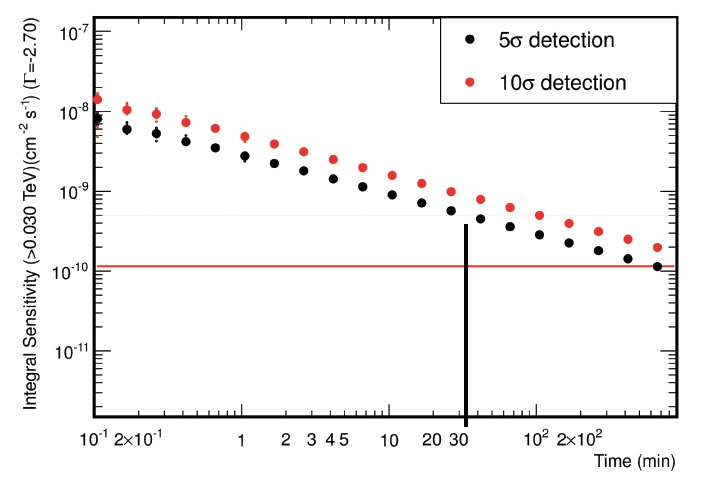
\includegraphics[width=0.75\textwidth]{Plots/cyg3-sens.png}
      }
      \only<2>{
      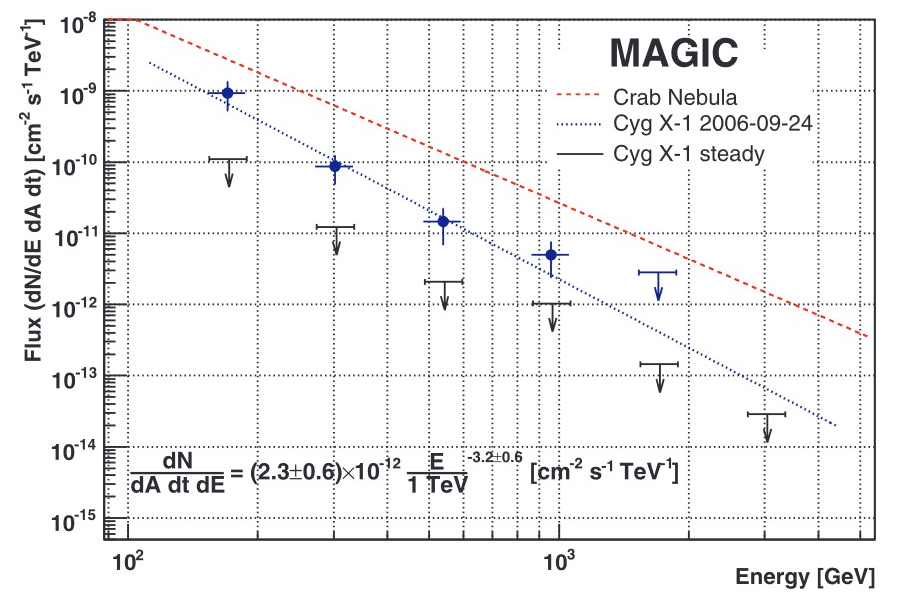
\includegraphics[width=0.75\textwidth]{Plots/cyg1-spectrum.png}
      }
    \end{minipage}
    \begin{minipage}{0.48\textwidth}
       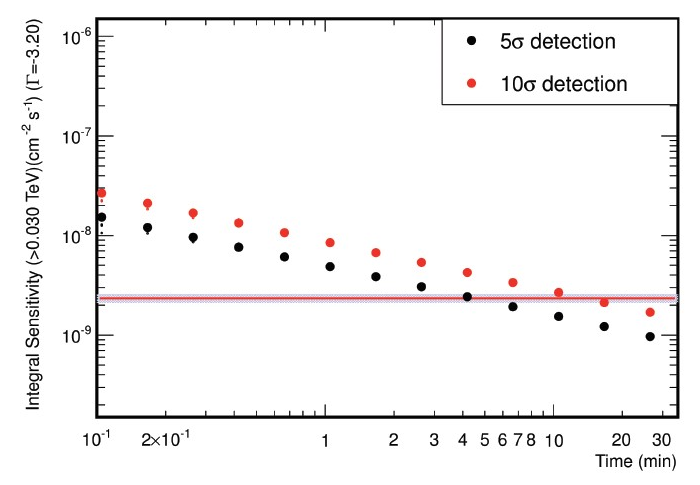
\includegraphics[width=0.75\textwidth]{Plots/cyg1-sens.png}
    \end{minipage}
    % \centering
    % \only<1>{
    % 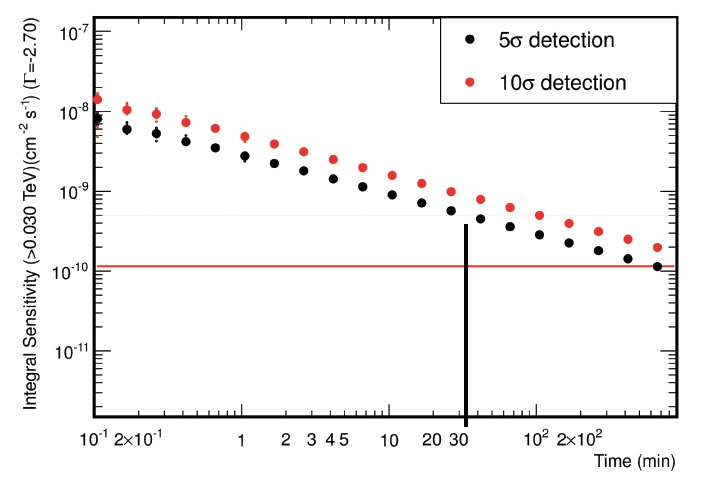
\includegraphics[width=0.38\textwidth]{Plots/cyg3-sens.png}
    % \hspace{0.5cm}
    % }
    % \only<2>{
    % 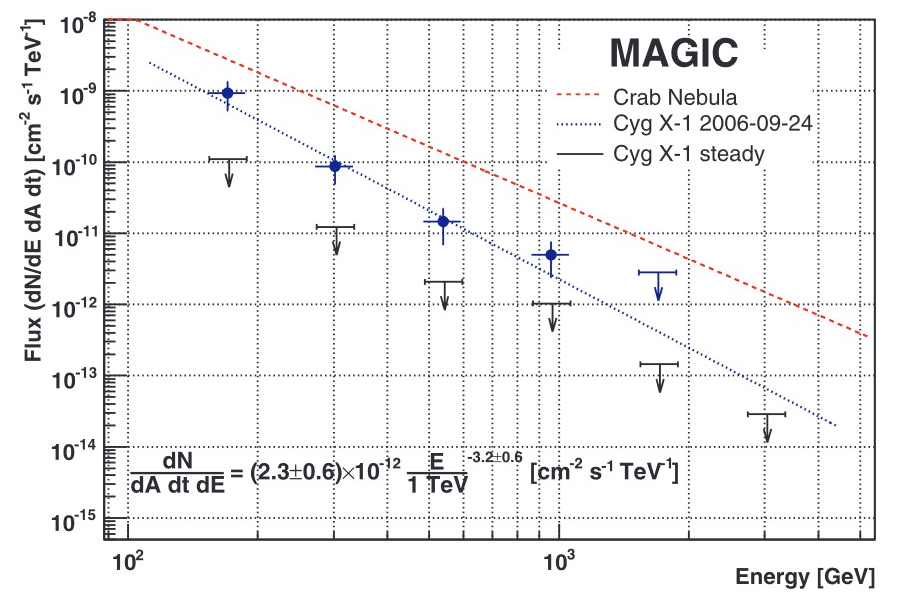
\includegraphics[width=0.38\textwidth]{Plots/cyg1-spectrum.png}
    % \hspace{0.5cm}
    % }
    % \onslide<1-2>
    % 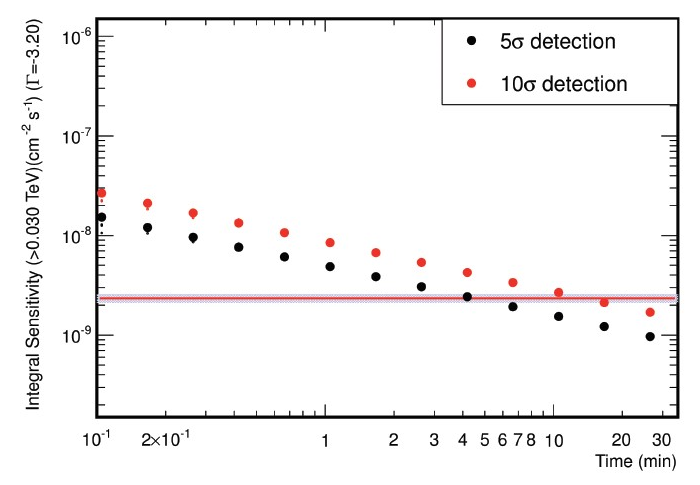
\includegraphics[width=0.38\textwidth]{Plots/cyg1-sens.png}
  \end{overprint}
\end{frame}

% ===============================================================================================================================
\begin{frame}{X-ray, optical, and radio transients}
  \begin{itemize}
    \item No simulations conducted due to exploration of predominantly new phase space
    \begin{itemize}
      \item [\to] Potential to provide high-impact results with moderate amount of observation time
    \end{itemize}
    \item Data products will be light curves and spectra or upper limits
  \end{itemize}
\end{frame}

% ===============================================================================================================================
\begin{frame}{HE neutrino transients}
  \begin{itemize}
    \item Detection of VHE gamma rays associated with HE neutrinos is critical to revealing and understanding HE neutrino sources
    \begin{itemize}
      \item [\to] Potential to unveil sources of UHECRs
    \end{itemize}
    \item Assumption, that detected neutrinos originate from $pp$ and $p\gamma$ interactions leads to time-averaged fluxes of
    \begin{center}
      \numrange{0.6}{1.7e8}\si{\giga\eV\centi\meter^{-2}\second^{-1}}
    \end{center}
    \begin{itemize}
      \item [\to] Neglects EBL attenuation
    \end{itemize}
    \item True flux can be higher or lower depending on transient duration and amount of sources
  \end{itemize}
\end{frame}

% ===============================================================================================================================
\begin{frame}{GW transients}
  \begin{columns}[T]
    \begin{column}{0.6\textwidth}
      \begin{itemize}%
        \item Test the compact binary merger model for short GRBs
        \begin{itemize}
          \item [\to] Possible discrimination between NS-NS or NS-BH progenitors
        \end{itemize}
        \item Good localisation would permit follow-up observations in various wavebands
        \begin{itemize}
          \item [\to] Optical observations to reveal redshift could help measure energetics of these mergers
        \end{itemize}
        \item Binary BH mergers will test models for associated electromagnetic emission
        \uncover<2->{
        \item NS mergers may induce off-axis high-energy emission due to fast mass ejection
        \begin{itemize}
          \item [\to] Opportunity to study particle acceleration
        \end{itemize}
        }
      \end{itemize}
    \end{column}%
    \uncover<2->{
    \begin{column}{0.38\textwidth}
      \centering
      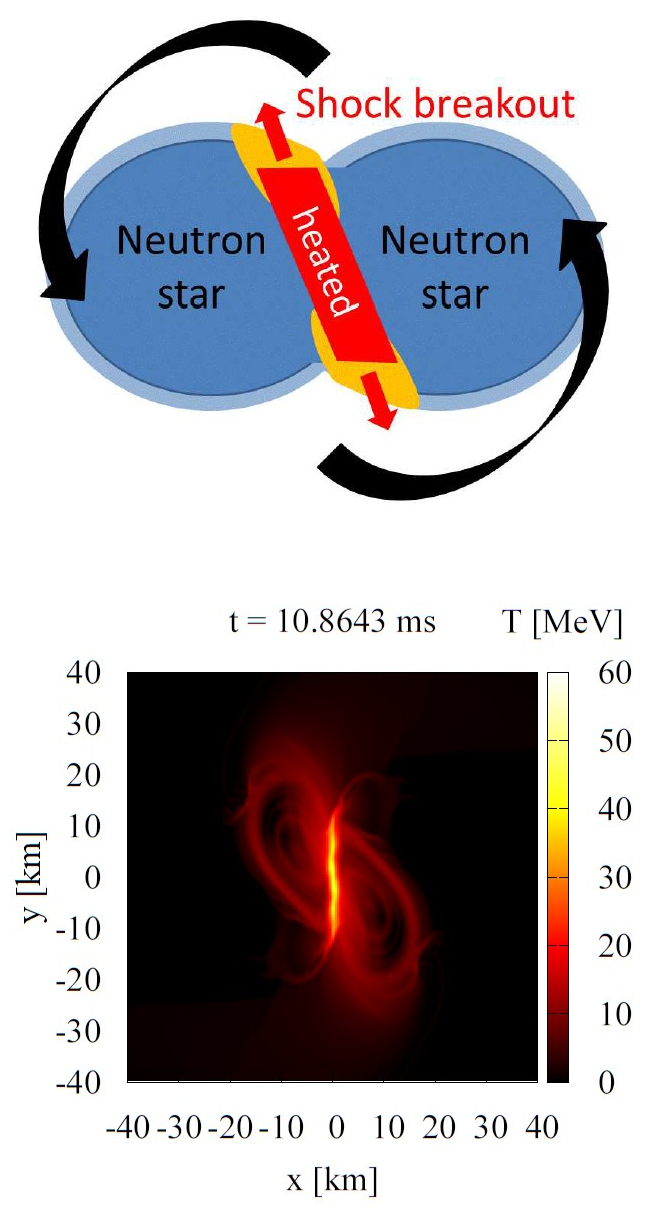
\includegraphics[height=\textwidth]{graphics/neutron-merger.png} % https://arxiv.org/abs/1209.5747v3
    \end{column}%
    }
  \end{columns}
\end{frame}

% ===============================================================================================================================
\begin{frame}{Serendipitous VHE transients}
  \begin{itemize}
    \item Limited knowledge so far, only approximate estimates for probability of detection possible
    \item Chances for serendipitous occurence of GRBs during normal pointing:
    \begin{itemize}
      \item [\to] LST, FoV of $\num{4.5}$ deg: once per $\sim\num{35}$ years
      \item [\to] MST, FoV of $\num{8}$ deg: once per $\sim\num{13}$ years
    \end{itemize}
    \item Detection rate may be increased with divergent pointing
    \uncover<2->{
    \item Prospects for flaring AGN depend on reached sensitivity of each observation, e.g. at sensitivity of $\SI{5}{\milli\crab}$:
    \begin{itemize}
      \item [\to] LST: $\numrange{2}{10}\si{\percent}$
      \item [\to] MST: $\numrange{6}{30}\si{\percent}$
    \end{itemize}
    \item Expectations for other types of serendipitous transients even more uncertain
    }
  \end{itemize}
\end{frame}

% ===============================================================================================================================
\begin{frame}{VHE transient survey}
  \begin{itemize}
    \item New limits on the VHE prompt emission of short GRBs
    \item Possible improvements for tests of LIV
    \item New discoveries are to be expected for high-energy properties of GRBs with lower luminosities
    \item MWL coordinated surveys with CTA could advance transient research, e.g. measurements of fast radio bursts
    \begin{itemize}
      \item [\to] Expectation of $\sim\num{2}$ FRBs per day in the FoV of CTA
    \end{itemize}
  \end{itemize}
\end{frame}
